% Options for packages loaded elsewhere
\PassOptionsToPackage{unicode}{hyperref}
\PassOptionsToPackage{hyphens}{url}
%
\documentclass[
]{book}
\usepackage{amsmath,amssymb}
\usepackage{lmodern}
\usepackage{ifxetex,ifluatex}
\ifnum 0\ifxetex 1\fi\ifluatex 1\fi=0 % if pdftex
  \usepackage[T1]{fontenc}
  \usepackage[utf8]{inputenc}
  \usepackage{textcomp} % provide euro and other symbols
\else % if luatex or xetex
  \usepackage{unicode-math}
  \defaultfontfeatures{Scale=MatchLowercase}
  \defaultfontfeatures[\rmfamily]{Ligatures=TeX,Scale=1}
\fi
% Use upquote if available, for straight quotes in verbatim environments
\IfFileExists{upquote.sty}{\usepackage{upquote}}{}
\IfFileExists{microtype.sty}{% use microtype if available
  \usepackage[]{microtype}
  \UseMicrotypeSet[protrusion]{basicmath} % disable protrusion for tt fonts
}{}
\makeatletter
\@ifundefined{KOMAClassName}{% if non-KOMA class
  \IfFileExists{parskip.sty}{%
    \usepackage{parskip}
  }{% else
    \setlength{\parindent}{0pt}
    \setlength{\parskip}{6pt plus 2pt minus 1pt}}
}{% if KOMA class
  \KOMAoptions{parskip=half}}
\makeatother
\usepackage{xcolor}
\IfFileExists{xurl.sty}{\usepackage{xurl}}{} % add URL line breaks if available
\IfFileExists{bookmark.sty}{\usepackage{bookmark}}{\usepackage{hyperref}}
\hypersetup{
  pdftitle={TILM 3701 - Tilastotiede ja Data 2022},
  pdfauthor={Koonneet; Henri Nyberg; Roope Rihtamo},
  hidelinks,
  pdfcreator={LaTeX via pandoc}}
\urlstyle{same} % disable monospaced font for URLs
\usepackage{longtable,booktabs,array}
\usepackage{calc} % for calculating minipage widths
% Correct order of tables after \paragraph or \subparagraph
\usepackage{etoolbox}
\makeatletter
\patchcmd\longtable{\par}{\if@noskipsec\mbox{}\fi\par}{}{}
\makeatother
% Allow footnotes in longtable head/foot
\IfFileExists{footnotehyper.sty}{\usepackage{footnotehyper}}{\usepackage{footnote}}
\makesavenoteenv{longtable}
\usepackage{graphicx}
\makeatletter
\def\maxwidth{\ifdim\Gin@nat@width>\linewidth\linewidth\else\Gin@nat@width\fi}
\def\maxheight{\ifdim\Gin@nat@height>\textheight\textheight\else\Gin@nat@height\fi}
\makeatother
% Scale images if necessary, so that they will not overflow the page
% margins by default, and it is still possible to overwrite the defaults
% using explicit options in \includegraphics[width, height, ...]{}
\setkeys{Gin}{width=\maxwidth,height=\maxheight,keepaspectratio}
% Set default figure placement to htbp
\makeatletter
\def\fps@figure{htbp}
\makeatother
\setlength{\emergencystretch}{3em} % prevent overfull lines
\providecommand{\tightlist}{%
  \setlength{\itemsep}{0pt}\setlength{\parskip}{0pt}}
\setcounter{secnumdepth}{5}
\usepackage{booktabs}
\usepackage{amsthm}
\makeatletter
\def\thm@space@setup{%
  \thm@preskip=8pt plus 2pt minus 4pt
  \thm@postskip=\thm@preskip
}
\makeatother

\usepackage{color}
\usepackage{framed}
\setlength{\fboxsep}{.8em}

\usepackage{tcolorbox}

\newtcolorbox{blackbox}{
  colback=black,
  colframe=orange,
  coltext=white,
  boxsep=5pt,
  arc=4pt}

%\newenvironment{infobox}[1]
%  {\begin{itemize}
%    \renewcommand{\labelitemi}{
%    \raisebox{-.7\height}[0pt][0pt]{
%      {\setkeys{Gin}{width=3em,keepaspectratio}
%        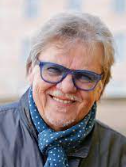
\includegraphics{images/mikko.PNG}}
%    }
%  }
%  \setlength{\fboxsep}{1em}
%  \begin{blackbox}
%  \item}
%  {
%  \end{blackbox}
%  \end{itemize}
%}
\usepackage{awesomebox}
\ifluatex
  \usepackage{selnolig}  % disable illegal ligatures
\fi
\usepackage[]{natbib}
\bibliographystyle{apalike}

\title{TILM 3701 - Tilastotiede ja Data 2022}
\author{Koonneet \and Henri Nyberg\footnote{Turun Yliopisto, matematiikan ja tilastotieteen laitos, \href{mailto:henri.nyberg@utu.fi}{\nolinkurl{henri.nyberg@utu.fi}}} \and Roope Rihtamo\footnote{Turun Yliopisto, matematiikan ja tilastotieteen laitos, \href{mailto:roope.rihtamo@utu.fi}{\nolinkurl{roope.rihtamo@utu.fi}}}}
\date{2022-08-22}

\begin{document}
\maketitle

{
\setcounter{tocdepth}{1}
\tableofcontents
}
\hypertarget{kurssin-rakenne}{%
\chapter*{Kurssin rakenne}\label{kurssin-rakenne}}
\addcontentsline{toc}{chapter}{Kurssin rakenne}

\begin{itemize}
\item
  Tällä kurssilla tarkoituksena on melko yleisellä tasolla johdatella tilastotieteen ja aineistojen (datan) maailmaan pohtimalla myös näiden laajempia merkityksiä tieteellisen tutkimuksen hyvin keskeisinä osina.
\item
  Kurssilla vältetään, mahdollisuuksien mukaan, kovin teknistä matemaattista esitystapaa, mutta tarvittavissa määrin tullaan myös käyttämään tilastotieteen perusopinnoissa tarvittavia matemaattisia merkintöjä ja määritelmiä. Esim. todennäköisyyslaskennan ja tilastollisen päättelyn perusteita ei käydä vielä riittävällä matemaattisella tarkkuudella lävitse, vaan nämä tarkastelut jäävät tätä kurssia seuraavien kurssien (\href{https://opas.peppi.utu.fi/fi/opintojakso/TILM3553/1734?period=2022-2024}{TILM3553 Todennäköisyyslaskennan peruskurssi} tai \href{https://opas.peppi.utu.fi/fi/opintojakso/TILM3568/3385?period=2022-2024}{TILM3568 Todennäköisyyslaskenta sivuaineopiskelijoille} sekä \href{https://opas.peppi.utu.fi/fi/opintojakso/TILM3555/1731?period=2022-2024}{TILM3555 Tilastollisen päättelyn peruskurssi}) asiaksi. Nämä kurssit, yhdessä alkuvaiheen pakollisten matematiikan kurssin lisäksi, muodostavat siis tämän kurssin johdannon kanssa lähtökohdan tilastotieteen opinnoille.
\item
  Luennot eivät suoraan perustu yhteen kirjaan tai lähteeseen. Käytettyjä lähdemateriaaleja luetellaan alapuolella oheislukemiston myötä.
\item
  Oheislukemistoa (sopivilta osin):

  \begin{itemize}
  \tightlist
  \item
    Mellin, I. (2004). Johdatus tilastotieteeseen: Tilastotieteen johdantokurssi (1.kirja). Yliopistopaino, Helsingin yliopisto.
  \item
    Mellin, I. (2000). Johdatus tilastotieteeseen: Tilastotieteen jatkokurssi (2.kirja). Yliopistopaino, Helsingin yliopisto.
  \item
    Mellin, I. (2006). Tilastolliset menetelmät. Luentomoniste, Aalto yliopisto (TKK).
  \item
    Holopainen, M. ja P. Pulkkinen (2008). Tilastolliset menetelmät. Sanoma Pro Oy.
  \item
    Pahkinen, E. ja R. Lehtonen (1989). Otanta-asetelmat ja tilastollinen analyysi. Gaudeamus, Helsinki.
  \item
    Pahkinen, E. ja R. Lehtonen (2004). Practical Methods for Design and Analysis of Complex Surveys. 2. painos, Wiley.
  \item
    Sund, R. (2003). Tilastotiede käytännön tutkimuksessa -kurssi. Helsingin yliopisto.
  \item
    Silver, N. (2014). Signaali ja kohina: Miksi monet ennusteet epäonnistuvat mutta jotkin eivät? Terra Cognita. (Suomentanut Kimmo Pietiläinen)

    \begin{itemize}
    \tightlist
    \item
      Englanninkielinen teos: Silver, N. (2015). The Signal and the Noise: Why So Many Predictions Fail--but Some Don't. Penguin Books; Illustrated edition
    \end{itemize}
  \item
    Pesonen, M. (2017). Kurssimateriaali kurssille Aineistonhankinta ja tutkimusasetelmat, Turun yliopisto.
  \item
    Vartia, Y. (1989). Tilastotieteen perusteet. Yliopistopaino, Helsinki. II painos.
  \end{itemize}
\item
  Muita taustamateriaaleja

  \begin{itemize}
  \tightlist
  \item
    \href{https://tilastokoulu.stat.fi/verkkokoulu_v2.xql?course_id=tkoulu_tilaj\&lesson_id=1\&subject_id=0\&page_type=sisalto}{Tilastokeskuksen tilastokoulu (linkki)}
  \item
    Tilastotieteen sanasto suomi-englanti-suomi, ks. Juha Alho, Elja Arjas, Esa Läärä ja Pekka Pere (2021). \href{https://tilastoseura.fi/}{Tilastotieteen sanasto. Suomen Tilastoseuran julkaisuja 8.}
  \end{itemize}
\end{itemize}

Suuret kiitokset Visa Kuntzelle ja Emil Lehdelle kommenteista ja avusta materiaalin työstämisessä. Kaikki jäljelle jääneet painovirheet ovat materiaalin kokoajien.

\hypertarget{johdantoa-ja-johdattelua-tilastotieteeseen}{%
\chapter{Johdantoa ja johdattelua tilastotieteeseen}\label{johdantoa-ja-johdattelua-tilastotieteeseen}}

\emph{Ihmisellä on luontainen pyrkimys ymmärtää, mitä hänen ympärillään tapahtuu. Ymmärrys perustuu ihmisen tekemiin havaintoihin, joita luokittelemalla tai seuraamalla hän pyrkii löytämään säännönmukaisuuksia. Näiden säännönmukaisuuksien löytäminen vaatii loogisten johtopäätösten tekoa. Pelkän uteliaisuuden tyydyttämiseen ja älyllisen mielihyvän lisäksi ihminen pyrkii ennakoimaan tulevaa ja siten varautumaan tuleviin tapahtumiin\ldots{} Edellä kuvattuja taitoja voi oppia.}

Holopainen ja Pulkkinen, 2008

\hypertarget{tilastotiede-ja-kurssin-idea}{%
\section{Tilastotiede ja kurssin idea}\label{tilastotiede-ja-kurssin-idea}}

\begin{itemize}
\tightlist
\item
  Tämän tilastotieteen ensimmäisen kurssin ideana on (ainakin)

  \begin{itemize}
  \tightlist
  \item
    Esitellä ja johdatella \textbf{tilastolliseen ja tieteelliseen ajatteluun} ja sen hyödyntämiseen eri tyyppisissä tutkimusongelmissa.
  \item
    Esitellä tilastotieteen roolia \textbf{empiirisen tutkimusaineiston keräämisessä ja analyysissä} sekä tarkastella tieteentekemisen ja tilastotieteen suhdetta.
  \item
    Pohtia \textbf{tilastotieteen olemusta tieteenalana} ja tarkastella tilastotieteen ja datatieteiden (data sciencen) samankaltaisuuksia ja eroja.
  \item
    Pohtia \textbf{sattuman ja satunnaisuuden roolia} jokapäiväisessä elämässä ja erityisesti osana tieteellistä tutkimusprosessia.
  \item
    Oppia tilastotieteen peruskäsitteitä ja (tilastollisen) tutkimuksenteon alkeita ja siihen liittyviä mahdollisia ongelmia esimerkiksi tilastollisten aineistojen keräämisessä.
  \item
    Oppia tilastollisten aineistojen \textbf{kuvaamisen ja käsittelyn} alkeita sekä tilasto(tieteellisen)llisen \textbf{mallintamisen} ja \textbf{koeasetelmien} peruskäsitteitä.
  \end{itemize}
\end{itemize}

\vspace{0.75cm}

\begin{itemize}
\tightlist
\item
  Kurssilla käsitellään myös \textbf{tilastollisen päättelyn} peruskäsitteitä ja perusteita kuten

  \begin{itemize}
  \tightlist
  \item
    Mitä on \textbf{todennäköisyys} ja miten sen tulkitaan tilastotieteessä sekä laajemmin tieteessä. Erityisesti tilastotieteen osalta keskiössä on tämän kurssin osalta \textbf{satunnaismuuttujat} sekä niihin liitettävät käsitteet

    \begin{itemize}
    \tightlist
    \item
      \textbf{Odotusarvo}, \textbf{varianssi} ja kahden (tai useamman) satunnaismuuttujan \textbf{korrelaatio}.
    \item
      Satunnaismuuttujien \textbf{todennäköisyysjakaumien} perusteita ja niiden yhteyksiä mm. normaalijakaumaan ja muutamiin muihin keskeisiin jakaumiin.
    \item
      Tilastollinen malli työkaluna satunnaismuuttujien formaalissa mallintamisessa ja päättelyssä. Tilastollisen malliin liittyy (usein) \textbf{parametreja} joihin tilastollinen päättely kohdistuu.
    \item
      Tilastollisten mallien \textbf{estimoinnin} perusidea, eli miten tilastollisen mallin parametreille muodostetaan arvot käytettävissä olevan aineiston pohjalta. Esimerkiksi: mitä tarkoittaa tilastollisen mallin parametrin \textbf{estimaattori} ja sen \textbf{harhattomuus}?
    \item
      Alustavia tarkasteluja tilastollisen mallin uskottavuuden käsitteelle ja \textbf{luottamusväleille} tilastollisen mallin estimoiduille parametreille.
    \end{itemize}
  \end{itemize}
\end{itemize}

\vspace{0.75cm}

\begin{itemize}
\tightlist
\item
  Toinen kurssin keskeisistä teemoista on tarkastella tieteellistä tutkimusprosessia teoriassa ja käytännössä. Tämä sisältää mm. seuraavia aiheita (joita siis käsitellään tällä kurssilla päällisin puolin ja varsin yleisestä näkökulmasta katsoen): tarkemmat yksityiskohdat jäävät tätä kurssia seuraavien tilastotieteen kurssien aihepiireiksi):

  \begin{itemize}
  \tightlist
  \item
    \textbf{Tutkimusongelman} asettaminen: mitä halutaan tutkia?\\
  \item
    Tutkimusongelman täsmentäminen ja \textbf{tutkimusstrategian} laatiminen: millä keinoin asetettuun tutkimusongelmaan voidaan vastata?
  \item
    \textbf{Tutkimusaineiston} (tai vain lyhyemmin \textbf{aineiston} eli \textbf{datan}) kerääminen

    \begin{itemize}
    \tightlist
    \item
      \textbf{Aineiston ennakkoehdot}: mitkä ehdot tulee täyttyä, jotta asetettuun tutkimusongelmaan voidaan vastata?
    \item
      \textbf{Otanta} (ja mittaaminen): miten tutkimusaineisto kerätään niin, että se täyttää aineiston ennakkoehdot? Erilaisissa tutkimuksissa käytetään erilaisia aineistoja kuten:

      \begin{itemize}
      \tightlist
      \item
        Survey- ja rekisteriaineistot
      \item
        Havaintoarvojen välistä korrelaatiota esiintyy mm. aikasarja-aineistojen tai pitkittäisaineistojen tapauksessa
      \end{itemize}
    \end{itemize}
  \end{itemize}
\item
  \textbf{Aineiston kuvaaminen}: minkälaista aineistoa on kerätty ja vastaako se ennakkoehtoja?
\item
  \textbf{Aineiston analyysin} lähtökohtia

  \begin{itemize}
  \tightlist
  \item
    Mitä tilastollista mallia/malleja käytetään?
  \item
    Mitä tarkoitetaan mallien tuntemattomien parametrien arvojen estimoinnilla?
  \item
    Tilastollinen päättely (estimointitulosten pohjalta)
  \end{itemize}
\item
  \textbf{Johtopäätelmien} tekeminen tilastollisen päättelyn pohjalta: saatiinko tutkimusongelmaan vastaus ja kuinka luotettava saatu vastaus on?
\end{itemize}

\hypertarget{tilastotieteen-asema-tutkimusyhteisuxf6n-ulkopuolella}{%
\section{Tilastotieteen asema tutkimusyhteisön ulkopuolella}\label{tilastotieteen-asema-tutkimusyhteisuxf6n-ulkopuolella}}

\begin{itemize}
\tightlist
\item
  Tilastotiede on oppiaineena usein varsin tuntematon toisen asteen opinnoista valmistuneelle, sillä sitä ei juurikaan opeteta lukioissa tai ammattikouluissa huolimatta sen keskeisestä ja kasvavasta roolista tiedemaailman kentillä.
\item
  Tiedeyhteisön ulkopuolellakin \textbf{tilastotiedettä ja tilastotieteilijöitä arvostetaan laajalti}.
\item
  \textbf{Tilastotiede onkin nostanut profiiliaan viimeisten vuosikymmenien aikana} tietoteknisen kehityksen tuotua laajat tietoaineistot ja kehittyneet laskennalliset menetelmät lähes jokaisen kansalaisen saataville.
\item
  Tämä ``datavallankumous'' näkyy tilastotieteilijöiden kysynnässä työmarkkinoilla: erilaisten aineistojen määrän lisääntyessä kasvaa myös kysyntä työntekijöistä, jotka osaavat ammatitaitoisesti käsitellä, tulkita ja mallintaa tilastollisia aineistoja.
\item
  Ei siis liene ihmekään, että erilaisten ``data''-alkuisten työpaikkojen, kuten \textbf{datatieteilijä} (eng. \textbf{data scientist}) tai \textbf{data-analyytikko} ( \textbf{data-analyst}) määrä on kasvanut voimakkaasti jo pidempään. Kaikkia tieto- ja datainensiivisten ammattien tekijöitä yhdistää yksi tekijä: \textbf{heidän tulee hallita ja osata tilastotiedettä!} Karkeistettuna mitä paremmin ja enemmän (laajemmin), sen parempi palkka ja monipuolisemmat työtehtävät!
\end{itemize}

\hypertarget{kurssin-luonne-tilastotieteen-ja-datatieteendata-analytiikan-opintojen-esittelijuxe4nuxe4}{%
\section{Kurssin luonne tilastotieteen (ja datatieteen/data-analytiikan) opintojen esittelijänä}\label{kurssin-luonne-tilastotieteen-ja-datatieteendata-analytiikan-opintojen-esittelijuxe4nuxe4}}

Kurssin mittaan esitellään tilastotieteen perusteiden lisäksi \textbf{miten TY:ssa tilastotieteen opinnoissa syvennytään} tällä kurssilla esiteltäviin menetelmiin, aineistotyyppeihin ja mallinnuskokonaisuuksiin.

\hypertarget{luku2}{%
\chapter{Tieteellinen tieto, tilastot ja arkitieto yhteiskunnassa}\label{luku2}}

\hypertarget{alaluku21}{%
\section{Mitä on tiede?}\label{alaluku21}}

\hypertarget{alaluku22}{%
\section{Tieteellinen menetelmä}\label{alaluku22}}

\hypertarget{alaluku23}{%
\section{Tilastojen yleisestä roolista yhteiskunnassa}\label{alaluku23}}

\hypertarget{alaluku24}{%
\section{Mitä on tutkimus?}\label{alaluku24}}

\hypertarget{alaluku25}{%
\section{Tieteellisen tutkimuksen vaiheet ja tulosten julkaiseminen}\label{alaluku25}}

\hypertarget{tilastotiede-tieteenalana}{%
\chapter{Tilastotiede tieteenalana}\label{tilastotiede-tieteenalana}}

Tässä luvussa hahmottelemme tilastotieteen piirteitä tieteenalana. Käymme läpi tilastotieteelle
ominaisia piirteitä, jotka erottavat sen niin lähitieteistä, kuten matematiikasta ja tietojenkäsit-
telytieteestä, kuin myös sovellusaloista. Usein näkee tilastotieteen typistettävän vain työkaluksi
eri sovellusalojen empiiriseen tutkimukseen siitäkin huolimatta että tilastotieteellä on oma rikas
teoriapohjansa sekä kiistaton asema omana tieteenalanaan.
Tieteenalan määritteleminen lyhyesti on aina hieman hankalaa. Tästä huolimatta seuraavassa
yritämme osaltaan vastata seuraaviin kysymyksiin:

\begin{itemize}
\tightlist
\item
  Mitä tilastotiede on ja mitä se ei ole? Miksi tilastotiede ei ole vain sovellettua matematiikkaa
  tai matematiikalla höystettyä tietojenkäsittelyä?
\item
  Mihin tilastotiedettä käytetään? Onko tilastotieteellä käyttöä ns. ``akatemian'' eli tutki-
  musyhteisön ulkopuolella?
\item
  Tilastotieteelle tyypillistä kritiikkiä?
\end{itemize}

\hypertarget{luku4}{%
\chapter{Sattuma ja satunnaisuus}\label{luku4}}

\hypertarget{alaluku41}{%
\section{Satunnaisilmiöt ja satunnaismuuttujat tilastotieteessä}\label{alaluku41}}

\hypertarget{alaluku42}{%
\section{Tilastotieteen suhde satunnaisuuteen ja todennäköisyyksiin}\label{alaluku42}}

\hypertarget{alaluku43}{%
\section{Tilastolliset mallit, jakaumat ja parametrit}\label{alaluku43}}

\hypertarget{alaluku44}{%
\section{Odotusarvo ja varianssi}\label{alaluku44}}

\hypertarget{alaluku45}{%
\section{Joitain jakaumia}\label{alaluku45}}

\hypertarget{normaalijakauma}{%
\subsection{Normaalijakauma}\label{normaalijakauma}}

\hypertarget{bernoulli--binomi--ja-poisson-jakauma}{%
\subsection{Bernoulli-, binomi- ja Poisson-jakauma}\label{bernoulli--binomi--ja-poisson-jakauma}}

\hypertarget{alaluku46}{%
\section{Sattuman rooli tieteenteossa: Vale-emävale-tilasto?}\label{alaluku46}}

\hypertarget{luku5}{%
\chapter{Tilastolliset aineistot, niiden kerääminen ja mittaaminen}\label{luku5}}

Edellisessä luvussa käsiteltiin tilastotieteen suhtautumista satunnaisilmiöihin. Tässä luvussa tarkastelemme lähemmin miten reaalimaailman satunnaisilmiöistä kerätään tietoa ja miten niitä voidaan mitata. Tilastotieteen perusoppimäärä rakentuu ajatukselle ilmiöiden tutkimisesta rajallisen ja epävarman tiedon vallitessa. Käytännössä tämä tarkoittaa sitä, että tutkimuksen kohteena olevat rajalliset aineistot sisältävät niin systemaattista kuin satunnaisuudesta johtuvaa vaihtelua. Tilastollisten menetelmien avulla pyrimme erottamaan systemaattisen vaihtelun satunnaisesta sekä tekemään tilastollista päättelyä aineiston generoimasta mekanismista. Lyhyesti tämä tarkoittaa aineiston systemaattisen vaihtelun tilastollista mallintamista ja sen parametrien estimointia otoksesta, joka kattaa vain (pienen) osajoukon koko populaation (perusjoukon) tilastoyksiköistä.

Voidaksemme tehdä uskottavaa päättelyä ``havainnoista parametreihin'', tulee otoksen olla riittävän \textbf{edustava}. Tämän luvun keskeisin oppi onkin, että miten otanta tulisi suorittaa, jotta havaintoaineisto olisi \textbf{edustava otos} populaatiosta, silloin kun aineisto kerätään otannalla. Vaikka aineiston hankinta vaatii yleensä runsaasti käytännön työtä, kannattaa se tehdä huolellisesti, sillä huonosti toteutetun otannan vuoksi tutkimusongelman kannalta keskeisiä johtopäätöksiä ei voida tehdä!

\hypertarget{alaluku51}{%
\section{Kertausta: Data eli aineisto}\label{alaluku51}}

\begin{itemize}
\item
  \textbf{Tilastollinen tutkimus} aloitetaan tutkimusaineiston keruun suunnittelulla.
\item
  Kertauksen vuoksi: tilastollinen tutkimusaineisto (havaintoaineisto) kostuu tilastoyksiköiden populaatiosta havaituista tilastoyksiköiden muuttujien arvoista.
\item
  Havaintoaineisto voidaan koota taulukoksi, johon listataan tilastoyksiköt riveille ja tilastomuuttujat sarakkeisiin. Jos havaintoaineisto koostuu \(n\) tilastoyksiköstä, joista jokaisesta on kerätty esim. \(m\) tilastomuuttujasta havainnot, niin havainnot voidaan kirjoittaa taulukon muotoon
\end{itemize}

Tässä siis rivillä \(i\) on \(i\). \textbf{tilastoyksikön} havainto ja \(j\) sarakkeessa on \(j\). tilastollisesta muuttujasta havaitut arvot \(x_{i,j}\). Ts. yhdellä rivillä on yhden tilastoyksikön tiedot kaikista tilastomuuttujista ja yksi sarake on kaikkien tilastoyksiköiden tiedot yhdestä tilastomuuttujasta.

\begin{itemize}
\item
  Usein (varsinkin parhaillaan kiihtyvällä vauhdilla) kerättävät havaintoaineistot ovat niin suuria, ettei edellisenkaltaisesta havaintotaulukosta voida usein suoraan tarkastelemalla nähdä aineiston pääpiirteitä.

  \begin{itemize}
  \tightlist
  \item
    Tällöin on tarpeen luokitella aineistoa taulukon muodostamiseksi.\\
  \item
    Luokittelussa on kysymys aineiston tiivistämisestä kohtuullisen kokoiseksi ja havainnollisempaan muotoon. Luokittelussa tilastomuuttujan arvot sijoitetaan eri luokkiin siten, että yhden tilastomuuttujan arvo voi kuulua vain yhteen luokkaan. Luokka ilmoitetaan yleensä luokkavälinä, kuten reaalilukuvälinä. Esimerkiksi henkilön ikä on tapana luokitella ikäjakauman kuvaamisessa 10-vuotisluokkiin (15-24, 25-34, \ldots), vaikka periaatteessa ikä voitaisiin ilmoittaa minuutinkin tarkkuudella.\\
  \item
    Luokkien lukumäärään vaikuttavat muun muassa tilastomuuttujan arvojen vaihteluväli ja havaintoaineiston laajuus. Luokittelussa pyritään siihen, että luokkien lukumäärä saadaan tarvittaessa luokkia yhdistämällä kohtuulliseksi ja että luokat valitaan tasavälisesti eli siten, että kahden peräkkäisen luokan alarajojen erotus on vakio. Kun aineistoa luokitellaan, aineiston luettavuus paranee mutta toisaalta osa tiedoista menetetään eivätkä yksittäiset havaintoarvot ole enää tiedossa.\\
  \item
    Emme vielä tällä kurssilla etene tämän pidemmälle tilastografiikan esittämisessä ja siihen liittyvissä pohdinnoissa. Muun muassa tilastollisen päättelyn peruskurssi (TILM3555) vastaa näihin kysymyksiin tarkemmin. Graafiset menetelmät ovat joka tapauksessa erittäin tärkeä osa aineiston havainnollistamista. Kuvat helpottavat aineiston tulkitsemista ja toimivat usein perusteltuna lähtökohtana monimutkaisempien tilastollisten mallien (ja algoritmien) sovittamiselle.
  \end{itemize}
\item
  Kvantitatiivisen tutkimuksen aineistoksi kelpaa periaatteessa kaikki havaintoihin perustuva informaatio, joka on \textbf{mittauksen} avulla muutettavissa numeeriseen muotoon.

  \begin{itemize}
  \tightlist
  \item
    Havaintoyksiköiden tilastollisten muuttujien numeerisia arvoja kutsutaan \textbf{havaintoarvoiksi} tai \textbf{havainnoiksi}.
  \item
    Kaikki havaitut tilastolliset muuttujat eivät ole aina mielenkiintoisia. Tutkimuksen kannalta mielenkiintoisia muuttujia kutsutaan \textbf{tutkimusmuuttujiksi}, joiden lisäksi havaintoaineisto pitää mahdollisesti sisällään \textbf{taustamuuttujia}.

    \begin{itemize}
    \tightlist
    \item
      Esimerkiksi, jos tutkimuksella halutaan tietoa suomalaisen aikuisväestön mielipiteistä, havaintoyksikköinä ovat aikuisväestöön kuuluvat henkilöt. Jos halutaan tietoa suomalaisista kunnista, havaintoyksikköinä ovat Suomen kunnat jne.
    \item
      Ensimmäisessä tapauksessa tilastollisina muuttujina on aikuisväestön mielipiteet, joita voidaan selvittää esimerkiksi kyselytutkimuksella. Toisaalta voidaan myös kerätä taustamuuttujiksi haastatelluista muita tietoja, kuten asuinpaikka, ikä ja ammatti.
    \end{itemize}
  \item
    Kaikkia mielenkiintoisia muuttujia ei kuitenkaan välttämättä voida havaita, eli niille ei voida määrittää numeerista arvoa.
  \item
    Tällöin puhutaan nk. \textbf{latenteista muuttujista}, eli muuttujista joita ei suoraan havaita mutta joiden oletetaan vaikuttavan havaittavien muuttujien taustalla. Latentteja muuttujia voidaan rakentaa tilastollisten mallien avulla käyttäen hyödyksi niihin liittyviä havaittuja muuttujia.
  \item
    Latentteja muuttujia ovat esimerkiksi elämänlaatu, onnellisuus, konservatiivisuus, yms.
  \end{itemize}
\item
  Tilastollinen tutkimus voi olla joko \textbf{kokonaistutkimus} tai \textbf{otantatutkimus}.

  \begin{itemize}
  \tightlist
  \item
    \textbf{Kokonaistutkimuksessa} tutkitaan kaikkia ajateltavissa olevia kohteita (kaikki perusjoukon alkiot tutkitaan).

    \begin{itemize}
    \tightlist
    \item
      Esimerkiksi jos tutkitaan Suomen kuntia, niin kokonaistutkimuksessa tutkitaan kaikki kunnat.
    \item
      Tai jos tutkitaan jonkin lääkeaineen vaikutuksia ihmisiin, niin tutkitaan jokainen ihminen erikseen. Selvää on, että tällainen kokonaistutkimus olisi liian vaikeaa toteuttaa.
    \end{itemize}
  \item
    \textbf{Otantatutkimuksessa} tutkimus kohdistetaan johonkin (populaation/perusjoukon) osajoukkoon ja johtopäätelmiä populaatiosta/perusjoukosta tehdään otokseen perustuen.

    \begin{itemize}
    \tightlist
    \item
      Perusjoukosta otokseen poimittuja alkioita kutsutaan \textbf{otosyksiköiksi} ja niiden muodostama osajoukko, eli \textbf{otos}, on se osa perusjoukkoa, joka tutkitaan tutkimusaineiston keräämisen jälkeen.
    \item
      Lääketutkimusta tehdäänkin poikkeuksetta otantatutkimuksena (ja kontrolloituina kokeina, ks. alempaa), jolloin lääkettä testataan vain osajoukolla koko ihmispopulaatiosta ja tämän osajoukon alkiot ovat otosyksiköitä.
    \item
      Näin toimimalla, ja riittävän edustavalla otoksella, saadaan kuitenkin tarpeeksi tietoa lääkeaineen vaikutuksista ja tulokset voidaan yleistää populaatiotasolle ja lääke ottaa käyttöön.
    \item
      Otantatutkimus on halvempi kuin kokonaistutkimus ja tulokset saadaan nopeammin!
    \end{itemize}
  \end{itemize}
\item
  Usein on kuitenkin niin, että koko populaation tutkiminen ei ole mahdollista tai kannattavaa. Tällöin tehtävä tutkimus on otantatutkimus ja tutkittavaksi valitaan perusjoukon osajoukko sopivaa \textbf{otantamenetelmää} (ks. alaluku \ref{alaluku55}) käyttäen.

  \begin{itemize}
  \tightlist
  \item
    Esimerkkinä aseiden patruunoita valmistava tehtailija, joka haluaisi tutkia toimivatko kaikki ammukset tai kaikkien suomalaisten haastatteleminen suomalaisten mielipiteitä kartoitettaessa. Myöskään valaisimien valmistaja tuskin tekee kokonaistutkimuksia valmistamiensa tuotteiden kestoajan selvittämiseksi.
  \end{itemize}
\item
  Tämän vuoksi useimmiten keskitytään perusjoukkoa edustavan pienemmän, mieluusti satunnaisesti valitun osajoukon eli \textbf{otoksen} tutkimiseen.

  \begin{itemize}
  \tightlist
  \item
    Otantatutkimuksissa tiedot kerätään useimmiten haastattelemella, kirjallisella/sähköisellä kyselyllä tai suoraan tietorekistereistä. Tiedonkeruun toteuttaminen (eri sovelluksissa) määrää osaltaan käytettävän otantamenetelmän.
  \item
    Teoriassa äärelliseen perusjoukkoon kohdistuvat kokonaistutkimukset voidaan aina tulkita otantatutkimuksiksi (perusjoukko tulkitaan otokseksi hypoteettisesta äärettömästä perusjoukosta)!

    \begin{itemize}
    \tightlist
    \item
      Esimerkiksi Galilein tekemät painovoiman vaikutusta kappaleiden putoamisaikaan liittyneet mittaukset. Koetuloksia (mittauksia) voidaan pitää otoksena äärettömästä mahdollisten koetulosten joukosta. Tällöin ainoa mahdollisuus ilmiön tutkimiseen on käyttää otantaa.
    \end{itemize}
  \end{itemize}
\item
  Otantatutkimuksen tulokset voivat olla luotettavampia kuin kokonaistutkimuksen.

  \begin{itemize}
  \tightlist
  \item
    Otantatutkimuksessa voidaan panostaa enemmän huolelliseen ja tarkkaan mittaamiseen sekä valitun otoksen tavoittamiseen.
  \item
    Kokonaistutkimuksessa vastauskato ja tarkasteltavan populaation valintavirhe ovat mahdollisia siinä kuin otantatutkimuksessakin.
  \end{itemize}
\item
  Otantateoria on yksi tilastotieteen keskeisimpiä oppeja ja tarjoaa teoreettisen kehikon empiiristen tutkimusten tulosten yleistämiseen. Tarkastellaan siis tarkemmin otannan ideaa ja toteuttamista seuraavassa alaluvussa.
\end{itemize}

\hypertarget{alaluku52}{%
\section{Otannan idea}\label{alaluku52}}

\hypertarget{alaluku53}{%
\section{Mittaaminen, mitta-asteikot ja tilastolliset muuttujat}\label{alaluku53}}

\hypertarget{alaluku54}{%
\section{Kontrolloidut kokeet ja suorat havainnot}\label{alaluku54}}

\hypertarget{alaluku55}{%
\section{Otantamenetelmät}\label{alaluku55}}

\hypertarget{yksinkertainen-satunnaisotanta}{%
\subsection{Yksinkertainen satunnaisotanta}\label{yksinkertainen-satunnaisotanta}}

\hypertarget{systemaattinen-otanta}{%
\subsection{Systemaattinen otanta}\label{systemaattinen-otanta}}

\hypertarget{ositettu-otanta}{%
\subsection{Ositettu otanta}\label{ositettu-otanta}}

\hypertarget{ryvuxe4sotanta}{%
\subsection{Ryväsotanta}\label{ryvuxe4sotanta}}

\hypertarget{alaluku56}{%
\section{Otantaesimerkkejä}\label{alaluku56}}

\hypertarget{alaluku57}{%
\section{Otannan haasteita vielä kootusti}\label{alaluku57}}

\hypertarget{luku6}{%
\chapter{Otokset ja otosjakaumat: tilastollisen päättelyn näkökulma}\label{luku6}}

\hypertarget{alaluku61}{%
\section{Satunnaisotos, yhteisjakauma ja tilastollinen malli}\label{alaluku61}}

\hypertarget{alaluku62}{%
\section{Otosjakauma: Estimaattori ja estimaatti}\label{alaluku62}}

\hypertarget{alaluku63}{%
\section{Otoskeskiarvo ja otosvarianssi (estimaattoreinta)}\label{alaluku63}}

\hypertarget{alaluku64}{%
\section{Suhteellisen frekvenssin otosjakauma}\label{alaluku64}}

\hypertarget{alaluku65}{%
\section{Muita tunnuslukuja}\label{alaluku65}}

\hypertarget{alaluku66}{%
\section{Luottamusvälit}\label{alaluku66}}

\hypertarget{alaluku67}{%
\section{Otoskoko}\label{alaluku67}}

\hypertarget{luku7}{%
\chapter{Tilastollinen riippuvuus ja korrelaatio}\label{luku7}}

\hypertarget{alaluku71}{%
\section{Muuttujien väliset riippuvuudet tilastollisen tutkimuksen kohteena}\label{alaluku71}}

\hypertarget{alaluku72}{%
\section{Kahden muuttujan havaintoaineiston kuvaaminen}\label{alaluku72}}

\hypertarget{alaluku73}{%
\section{Tunnusluvut}\label{alaluku73}}

\hypertarget{alaluku74}{%
\section{Satunnaismuuttujien kovarianssi ja korrelaatio}\label{alaluku74}}

\hypertarget{luku8}{%
\chapter{Regressioanalyysi}\label{luku8}}

\hypertarget{alaluku81}{%
\section{Johdatus regressioanalyysin ideaan}\label{alaluku81}}

\hypertarget{alaluku82}{%
\section{Yhden selittäjän lineaarinen regressiomalli}\label{alaluku82}}

\hypertarget{alaluku83}{%
\section{Muita regressiomalleja}\label{alaluku83}}

\hypertarget{luku9}{%
\chapter{Tilastotieteen rooli uuden tiedon tuottamisessa}\label{luku9}}

\hypertarget{alaluku91}{%
\section{Tilastollisen tutkimuksen yhteisiä elementtejä}\label{alaluku91}}

\hypertarget{alaluku92}{%
\section{Tutkimusprosessi}\label{alaluku92}}

\hypertarget{luku10}{%
\chapter{Aineisto- ja tutkimustyypit ja koeasetelmat}\label{luku10}}

\hypertarget{alaluku101}{%
\section{Tutkimustyypit}\label{alaluku101}}

\hypertarget{alaluku102}{%
\section{Tutkimusstrategiat}\label{alaluku102}}

\hypertarget{alaluku103}{%
\section{Erilaisia aineistoja ja aineistolähteitä}\label{alaluku103}}

\hypertarget{alaluku104}{%
\subsection{Rekisteriaineistot}\label{alaluku104}}

\hypertarget{alaluku105}{%
\subsection{Aikasarjat ja paneeliaineistot}\label{alaluku105}}

\hypertarget{alaluku106}{%
\subsection{Survey eli haastattelu- tai kyselytutkimus}\label{alaluku106}}

\hypertarget{luku11}{%
\chapter{Tilastollisesta ennustamisesta}\label{luku11}}

\hypertarget{alaluku111}{%
\section{Tilastollinen selittäminen vs.~ennustaminen}\label{alaluku111}}

\hypertarget{alaluku112}{%
\section{Tilastolliseen ennustamiseen liittyviä huomioita}\label{alaluku112}}

\hypertarget{luku12}{%
\chapter{Tilastotieteen kehityksen nykytrendejä}\label{luku12}}

  \bibliography{book.bib,packages.bib}

\end{document}
